Here you can see how to include an image in your document.


% ############### PRODUCT PERSPECTIVE ####################à
\subsection{Product perspective}
DREAM is a functional multi-user software platform which purpose is to provide functionalities described in section \ref{sect:product_functions}. The system will be composed by a series of software and hardware interfaces that interact in such a way to let users manipulate shared data. It also will exploit some graphical interface packages in order to be user friendly and easy to use.

\begin{figure}[H]
	\centering
    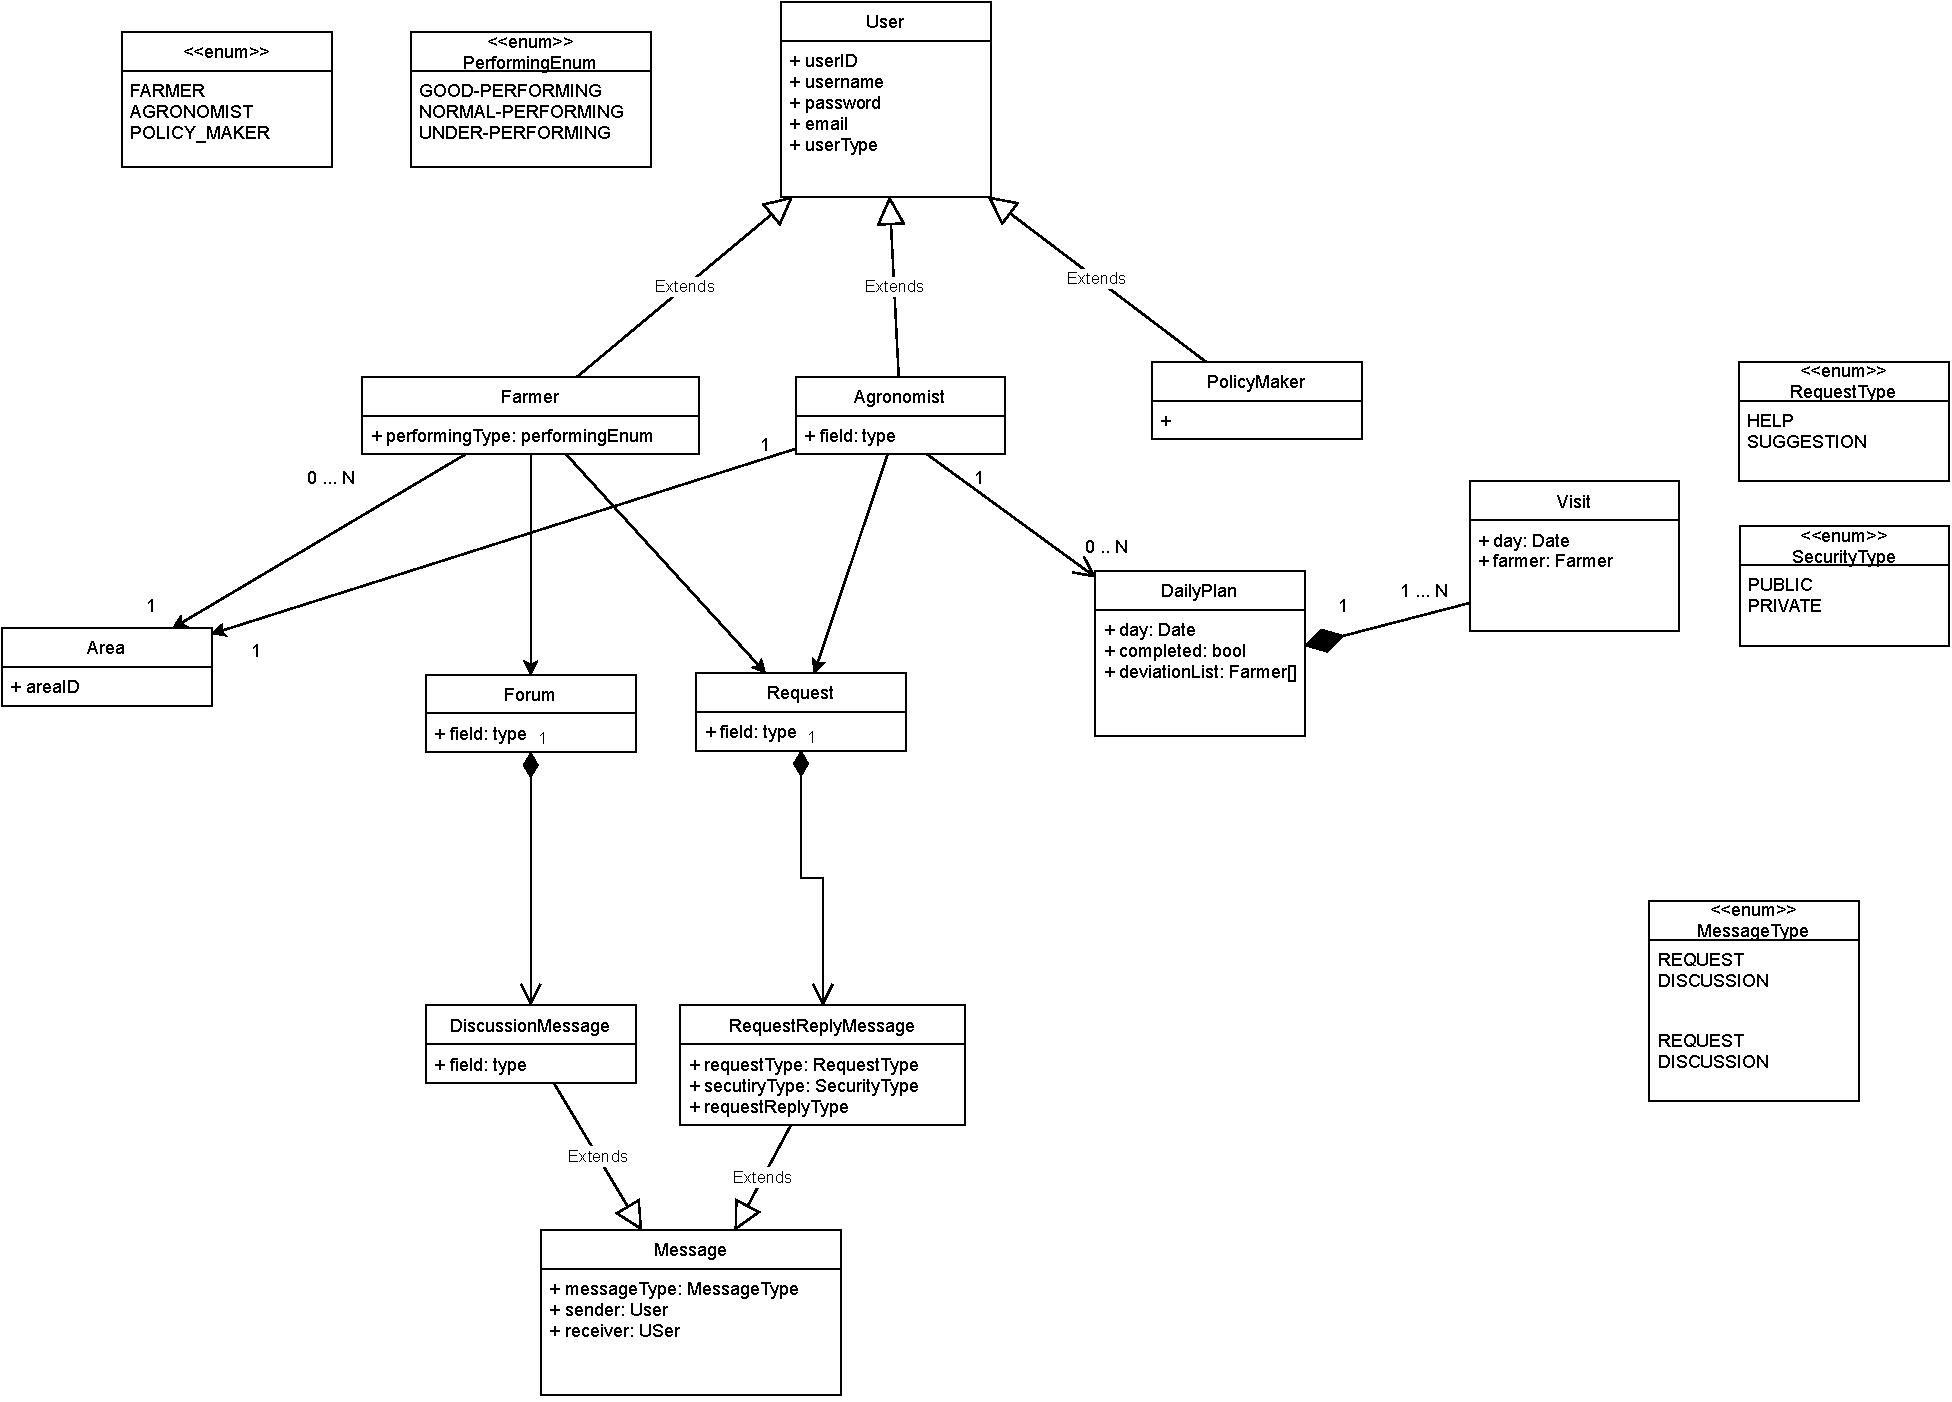
\includegraphics[page=1, width=\textwidth]{Images/SE2 - class diagram.pdf}
	\caption{\label{tab:class_diagram}High level UML diagram}
\end{figure}

\subsubsection{User interfaces} % TODO revise te verbs
\label{sect:user_interfaces}
According to the assignment document the system will interact with 3 different user classes: policy makers, farmers and agronomists. In order to be more accessible and to fulfill the above mentioned professional figures needs the application will be supported by different devices. These users should interface to the service through electronic devices with an internet connection. Users that needs to access the service will have the possibility to connect throught:
\begin{itemize}
    \item an internet browser, addressing a specific web domain (such as \textit{www.dream.com}) that permits users to sign up/in a dedicated web application;
    \item a mobile application that can be installed on smartphones (both IOS and Android).
\end{itemize}


\subsubsection{Software interfaces}
In order to improve software flexibility and quality DREAM will use a set of external software interfaces. Rather than providing specific services names, we consider reasonable referring to them as functionalities to then be specified in design phase:
\begin{description}[font=~\normalfont\scshape]
    \item[\textbf{\textcolor{myblue}{universal logins}}] \hfill \\login APIs that also provide access by using their Facebook, Twitter, or Google profile login details are good candidates in order to quickly autenthicate the user while guaranteeing security;
    \item[\textbf{\textcolor{myblue}{big data manipulation}}] \hfill \\since a wide quantity of information needs to be recorded and accessed in a distributed system fashion, DBMS APIs are necessary for data extraction performances optimization;
    \item[\textbf{\textcolor{myblue}{third party payment processing}}] \hfill \\for guaranteeing secure payment transactions online payment APIs such as PayPal should be used;
    \item[\textbf{\textcolor{myblue}{third party data science research}}] \hfill \\% TODO
\end{description}

\subsubsection{Hardware interfaces \& constraints}
DREAM system will be composed by multiple different hardware components which can be described from two points of view:
\begin{description}[font=~\normalfont\scshape]
    \item[\textbf{\textcolor{myblue}{user perspective}}] \hfill \\Since DREAM platform is accessed by users in a fully virtual way, hardware interfaces that provides internet connection, input components, a screen to visualize GUI and a web browser or an application store are required (like smartphones, personal computers, tablets and smart TVs).
    \item[\textbf{\textcolor{myblue}{system perspective}}] \hfill \\According to the assignment, the system should be composed by hardware devices designed to gather Telangana's environment information such as soil humidity sensor and the ones responsible for the predefined water irrigation system.
\end{description}
The user hardware interfaces also represent constrains that are required in order to permit the users to interact with the systems and manipulate shared data.

\subsection{Product functions}
\label{sect:product_functions}
In this section the main functionalities of the S2B are presented, described and enriched with BPMN diagrams in order to guarantee an higher level of understanding.
\subsubsection{Sign up}

\subsubsection{Sharing issues to get help, suggestions}

\subsubsection{Communication(among farmer) on forum}
\subsubsection{Visits low performer}
\subsubsection{Visualize the performance data}


\subsection{Actors}
\subsubsection{User}
It is a person who wants to use the service. In order to access the system, it has to register to the platform (the first time) and be logged in (the following times). It also requires an Internet connection to properly use the system.
\subsubsection{Policy maker}
It is someone interested in the overall performing situation of Telangana’s farmers (e.g., Telangana’s government). It is able to surf on DREAM’s website. It uses the service to visualise information about well and under-performing farmers and to understand if the steering initiatives are producing significant results.
\subsubsection{Farmer}
It is a farmer of Telangana. It is able to surf on DREAM’s website (or to use the smartphone application). It uses the service in order to discuss with other farmers, to send requests for help to an agronomist, to insert information about what / how much he is producing, to know when he will receive a visit from an agronomist. It takes advantage in using the system because it receives incentives if he is well-performing or receives help if he is under-performing.
\subsubsection{Agronomist}
It is an agronomist of Telangana. It is able to surf on DREAM’s website (or to use the smartphone application). It uses the service to answer farmers' requests for help, to visualise data concerning their area (weather forecasts, well and under-performing farmers), to visualise and update a daily plan to visit farms in the area, to confirm the execution or specify deviation from the daily plan.


\subsection{Assumptions, dependencies and constraints}

\begin{sidewaysfigure}
\centering
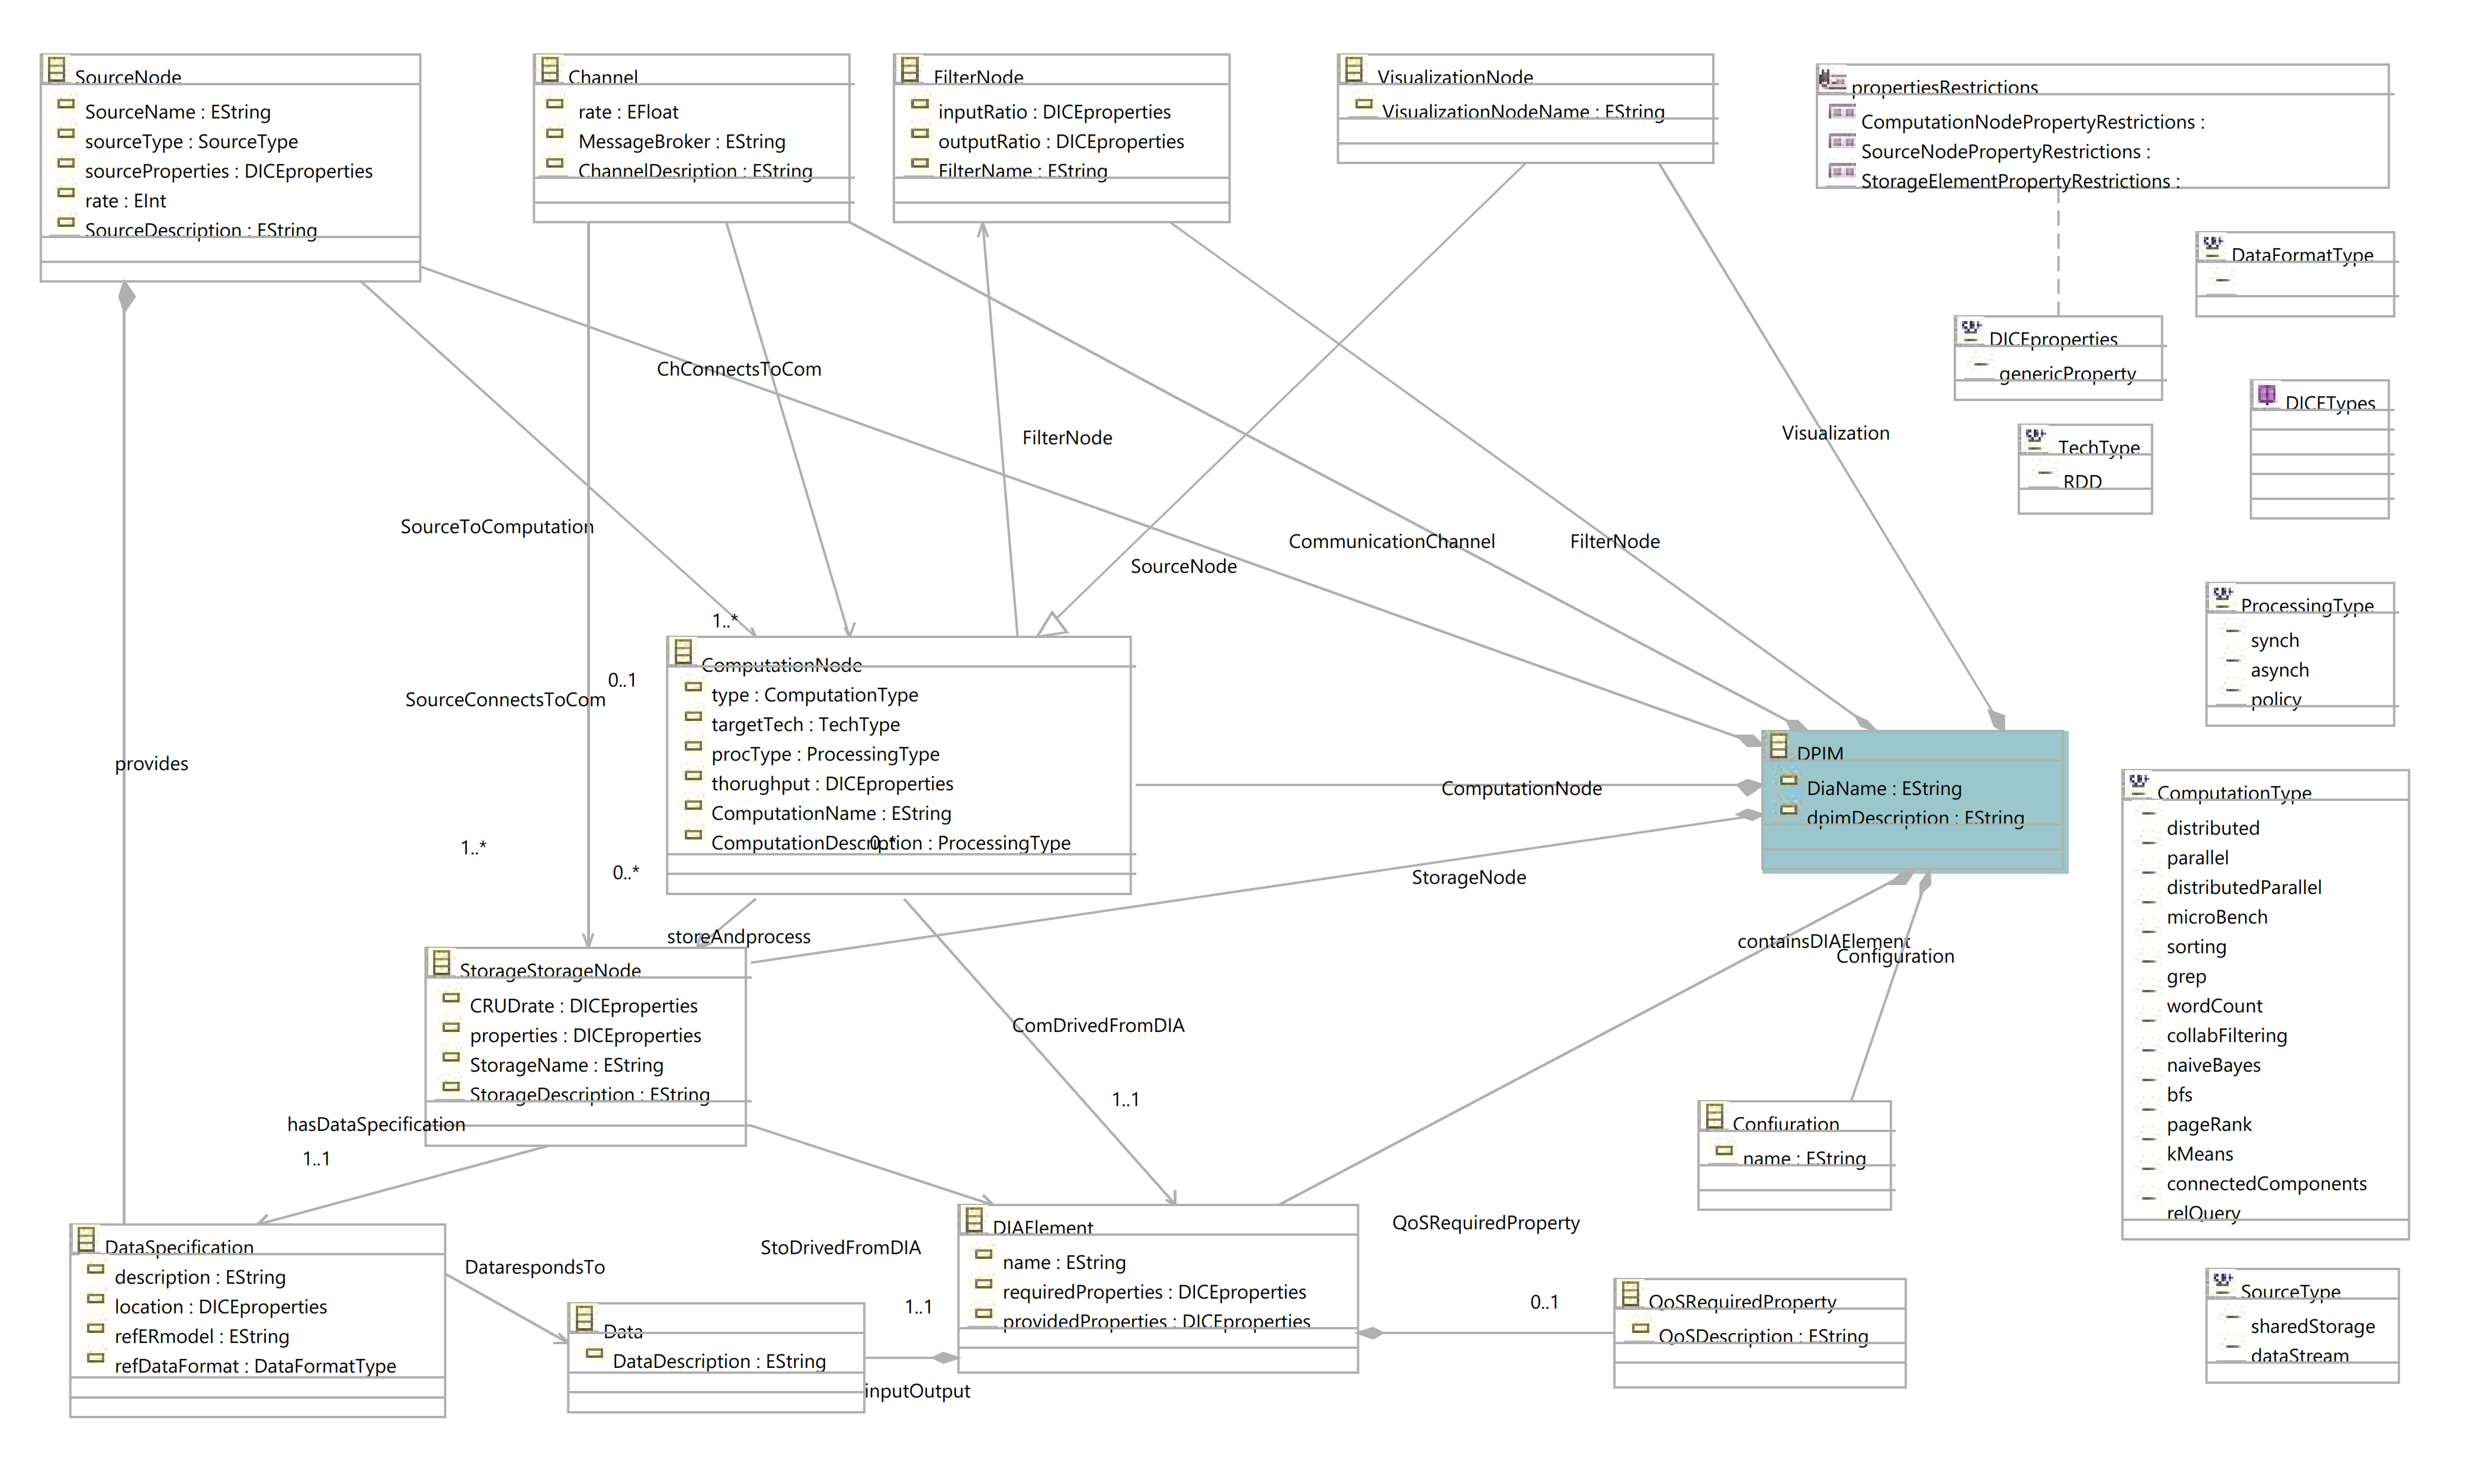
\includegraphics[width=\textwidth]{Images/11.png}
\caption{\label{fig:metamodel}DICE DPIM metamodel.}
\end{sidewaysfigure}

\begin{figure}
\centering
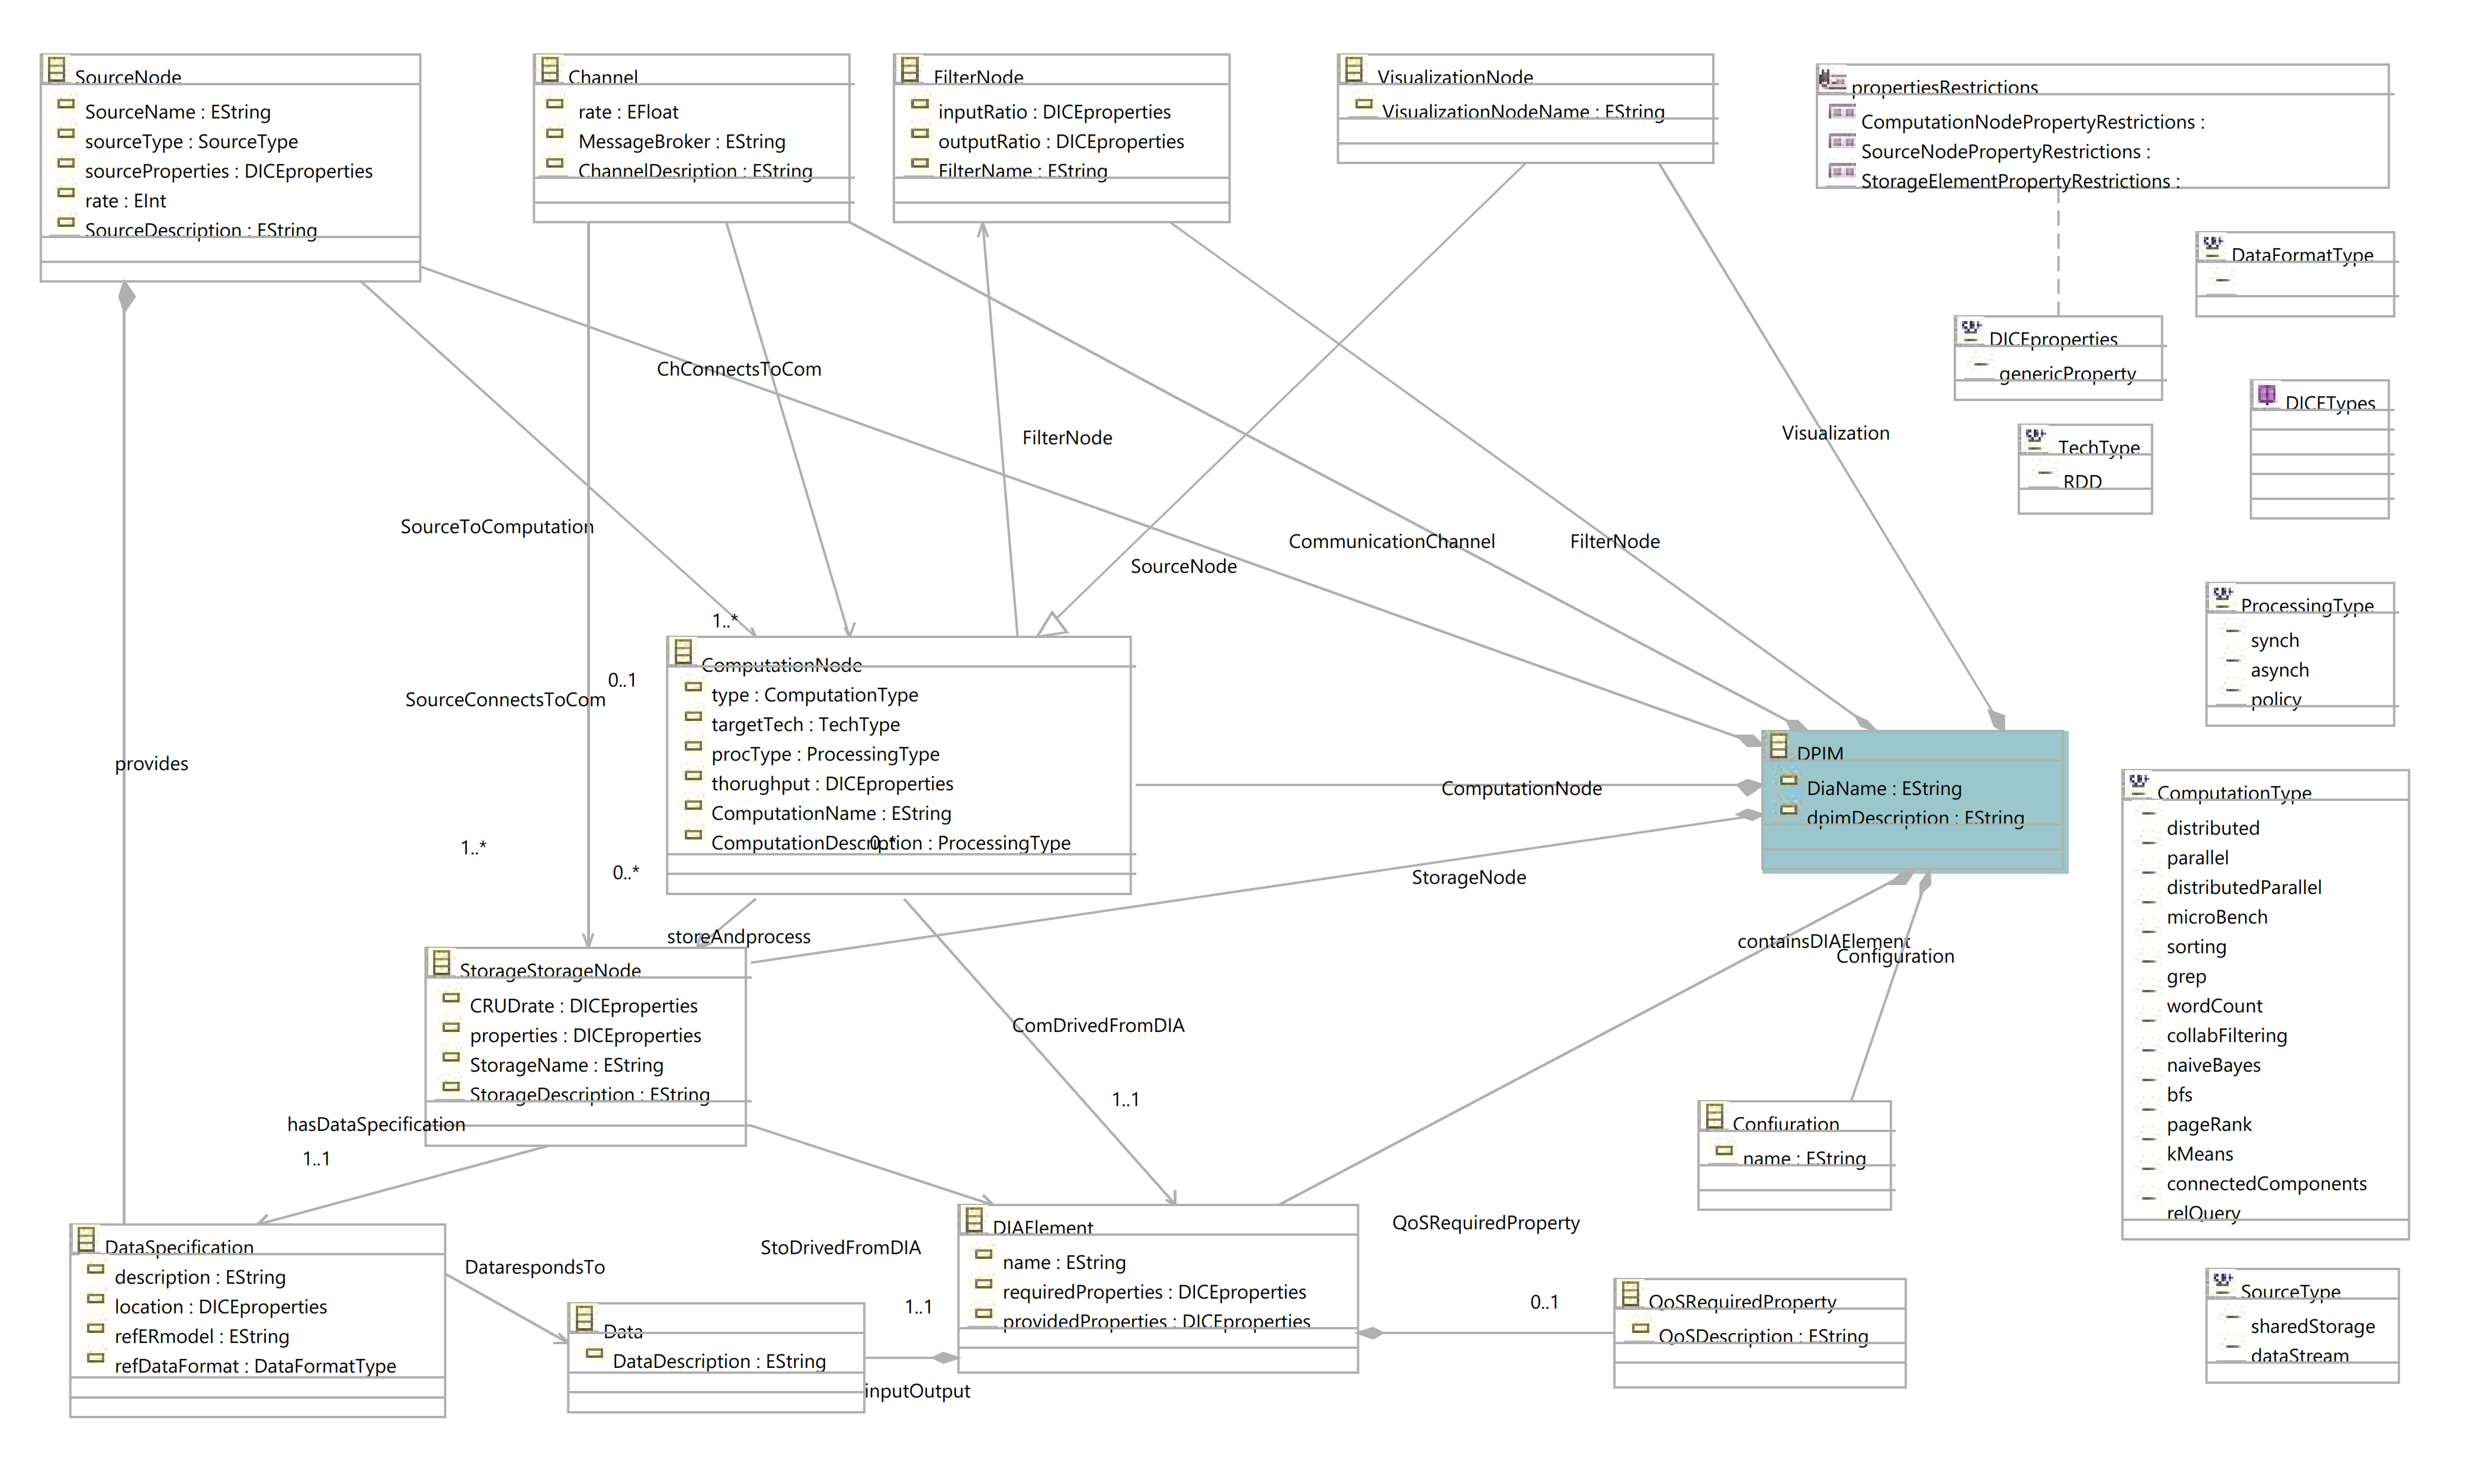
\includegraphics[width=\textwidth]{Images/11.png}
\caption{\label{fig:metamodel2}DICE DPIM metamodel in portrait form.}
\end{figure}

Here is the command to refer to another element (section, figure, table, ...) in the document: \emph{As discussed in Section~\ref{sect:overview} and as shown in Figure~\ref{fig:metamodel}, ...}. Here is how to introduce a bibliographic citation~\cite{DAM}. Bibliographic references should be included in a \texttt{.bib} file. 

Table generation is a bit complicated in Latex. You will soon become proficient, but to start you can rely on tools or external services. See for instance this \href{https://www.tablesgenerator.com}{https://www.tablesgenerator.com}. 
